\documentclass[12pt]{exam}
% \usepackage{pslatex}
\usepackage{graphicx}
\DeclareGraphicsExtensions{.jpg}
\usepackage{amsmath}
\usepackage{amsfonts,eucal}
\usepackage{enumerate}
\firstpageheader{}{}{}
\runningheader{\textbf{Math 251: Fall 2012}}
 {\ifcontinuation{\textbf{Problem continues}}{}}
 {\emph{Page \thepage~of \numpages}}
\runningheadrule
\runningfooter{}{\ifincomplete{continues on next page}{}}{}
\setlength{\parskip}{1.2ex}
\setlength{\parindent}{0pt}
\pagestyle{headandfoot}
\newcommand{\N}{\mathbf{N}}
\newcommand{\Z}{\mathbf{Z}}
\newcommand{\R}{\mathbf{R}}
\DeclareGraphicsExtensions{.pdf,.png,.jpg}
\renewcommand{\vec}[1]{\mathbf{#1}}
\begin{document}

% \printanswers
\addpoints

\noindent
\textbf{{\large Mathematics 251 \\ Final Exam}}
% \hfill Name: \underline{\hspace{0.5in}Answers\hspace{2in}}

\noindent
December 10, 2012  \hfill Name: \underline{\hspace{3in}}

\noindent
\textbf{Instructions}: This exam is closed book: you may refer to one double-sided $8.5 \times 11$ page of handwritten notes, but no electronic aids or
other printed references are permitted. \emph{Justification of all answers is required
for partial credit.} Unless
specifically directed, leave all answers in \textbf{exact form}, e.g.\
$\sqrt{3}$ instead of~1.732 and $\pi/2$ instead of~$1.57$.

Show all pertinent work. \emph{Correct answers without accompanying work will receive little or no credit.} Results from homework or from class can be cited freely. It is in your interest to display your solution in a
clear, readable fashion. Note that standards of justification are not as high as for homework.

\emph{Budget your time wisely.} It is a good idea to look through the entire exam before beginning work on a particular problem.

If your work continues onto the back of another page, please indicate
this. Check and make sure you have all of the pages in the
exam; there should be \numpages, including this one. If you have a
question, please raise your hand.

Be sure to read all questions carefully and completely.

\vspace*{1.0in}

\begin{center}
\partialgradetable{range1}[h] % was \partialcombined...

\partialgradetable{range2}[h]
\end{center}

\vspace*{0.5in}

\begin{center}
{\Large \emph{Good luck!}}
\end{center}

\newpage

\begin{questions}
    \begingradingrange{range1}
    \question[16] Please find the indicated partial derivatives.

        \begin{parts}
            \part $f(x,y) = x^4 y^3$; find $f_x$, $f_y$.
            \part $w = \dfrac{x}{(x^2+y^2+z^2)^{3/2}}$; find $\partial w / \partial x$.
            \part $z = \dfrac{y^2}{1+y^2}$; find $\partial z / \partial x$.
            \part $u = 3x^2 y - 6xy^4$; find $u_{xx}$ and $u_{yy}$.
        \end{parts}

    %\question[16]
    %
    %    Find the linearization $L(x,y,z)$ of the function $f(x,y,z) = xy/z$ at $(2,1,2)$. Use it to estimate the value of $f(2.05,0.9,2.01)$.

    \question In this problem, consider the function~$g(x,y) = 7 - 2xy^2$ and the point~$P = (1,-1)$. 

    \begin{parts}
        \part[12] Give a formula for the linearization~$L(x,y)$ of~$g$ at~$P$. Describe the geometric relationship between the graphs of the two functions $L(x,y)$ and $g(x,y)$ (in complete sentences).

        \part[4] Use the linearization to estimate~$g(0.9, -1.1)$.
    \end{parts}

    \question[16] Verify that $(1,1,1)$ is the center of mass of the tetrahedron bounded by the planes $x = 0$, $y = 0$, $z = 0$, and $x + y + z = 4$, assuming uniform (constant) density. \emph{Hint.} You are allowed to refer to the symmetries of the problem and draw conclusions from them. However, arguments that do not involve an integral will receive little to no credit.

    \question[16] \textbf{NOTE:} the parts of this problem are unrelated.
    \begin{parts}
        \part Calculate $\dfrac{d}{dt}f(\vec{r}(t))$, where
        \[
            f(x,y) = \sin(xy), \; \vec{r}(t) = \langle e^{2t}, e^{3t} \rangle.
        \]
        \part Calculate the directional derivative of $g(x,y) = x^2 + y^3$ in the direction of $\vec{v} = \langle 4, 3 \rangle$ at $P = \langle 1, 2 \rangle$.
    \end{parts}

    \question This problem concerns the cycloid described by the vector-valued function
    \[
        \vec{r}(t) = \langle x(t), y(t) \rangle = \langle t - \sin t, 1 - \cos t \rangle.
    \]
    \begin{parts}
        \part[6] Find the tangent vector $\vec{r'}(t)$ of a particle whose position vector is $\vec{r}(t)$.
        \part[6] Verify that the curvature of the cycloid at the point given by $t = \pi$ is $\kappa (t) = 1/4$.
        \part[4] Give parametric equations for the tangent line to the cycloid at $\vec{r}(\pi/2) = (1,1)$.
    \end{parts}

    \endgradingrange{range1}
    \begingradingrange{range2}

    \question[16] \label{prob:planepic}
        Find an equation for the plane pictured (last page). \emph{Hint.} Begin by finding a vector normal to the plane.
        
   \question[16]
        Among all lidless boxes (i.e., five sides, no top) of volume 27, find the one with minimum surface area. Make sure to justify why your answer is a minimum, paying particular attention to boundary points.

    
    %\question[8]
    %    Find the center of mass of the tetrahedron bounded by the planes $x = 0$, $y = 0$, $z = 0$, and $2x+3y+6z = 6$. Assume the solid has uniform density. \emph{Hint.} Draw a picture. Find the coordinates of all the corners of the tetrahedron.

    \question[16]
        Sketch the domain of integration. Then change the order of integration and evaluate the integral (in the new order you just found---it is known that this integral is impossible to evaluate in the order given).
        \[
            \int_0^4 \int_{\sqrt{y}}^2 \sqrt{x^3 + 1} \; dx \; dy
        \]

    \question[8] \label{prob:polar}
        \textbf{Using polar coordinates,} express the area of the pictured region (below) as an integral or as a sum of integrals. Solutions not making use of polar coordinates will not receive much credit. \textbf{Do NOT evaluate your integrals.} \emph{Hint}. The smaller circle has rectangular equation $(x-1)^2 + y^2 = 1$. Start by converting this equation to polar form.
        
    \question At a certain moment, a moving particle has velocity $\vec{v} = \langle 1, 0, 1 \rangle$ and acceleration $\vec{a} = \langle 2, 1, -3 \rangle$.
        \begin{parts}  

             \part[6]
             Find the unit tangent vector $\vec{T}$ at this moment.
             \part[4]
             Find the unit normal vector $\vec{N}$ at this moment, and give the components of acceleration in the tangent and normal directions (the coefficients in the equation $\vec{a} = a_{\vec{T}} \vec{T} + a_{\vec{N}} \vec{N}$).
             \part[4]
             Is the particle speeding up or slowing down at this moment? Why?
             %\bonuspart[6]
               
        \end{parts}

        \endgradingrange{range2}

        \end{questions}

        %\newpage

        \begin{figure}[ht]
            \centering
            \begin{minipage}[t]{0.45\linewidth}
                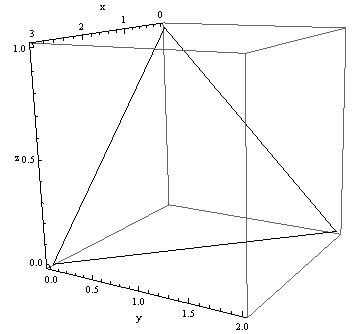
\includegraphics[height=180pt,width=167pt]{f12_final_fig1}
                \caption{Problem \ref{prob:planepic}. Be cautious in interpreting the labels on the axes.}
            \end{minipage}
            \hspace{0.05\linewidth}
            \begin{minipage}[t]{0.45\linewidth}
            \centering
                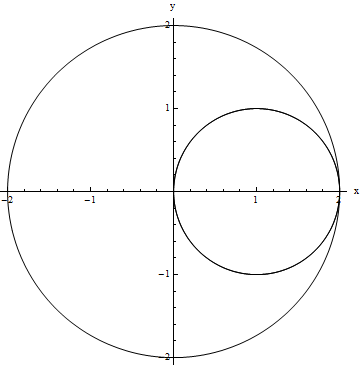
\includegraphics[height=180pt,width=182pt]{f12_final_fig2}
                \caption{Problem \ref{prob:polar}.}
            \end{minipage}% \end{figure}
        \end{figure}

\end{document}